\documentclass[11pt]{article}
\title{Usage Trend of Common Statistical Methods in Scientific Papers \vspace{-2ex}}
\date{\vspace{-5ex}}
\author{Gege Gui}
\usepackage{geometry,amsmath,amssymb, graphicx}
\usepackage{float}
\usepackage{lipsum}
\usepackage{enumitem}
\usepackage{adjustbox}
\usepackage{multirow}
\usepackage{hhline}
\usepackage{epstopdf}
\usepackage{fullpage}
\usepackage[utf8]{inputenc}
\usepackage[demo]{graphicx}
\usepackage{caption}
\usepackage{subcaption}
\usepackage{sectsty}
\sectionfont{\fontsize{15}{15}\selectfont}
\subsectoinfont{\fontsize{12}{12}\selectfont}
\usepackage{titlesec}
\titlespacing\section{0pt}{0pt plus 0pt minus 0pt}{0pt plus 0pt minus 0pt}
\newlist{steps}{enumerate}{1}
\setlist[steps, 1]{label = Step \arabic*:}
\usepackage[parfill]{parskip}
\renewcommand{\multirowsetup}{\centering}
\begin{document}
\maketitle
\newcommand{\code}[1]{\texttt{#1}}
\newcommand{\Var}{\mathrm{Var}}
\newcommand{\logit}{\mathrm{logit}}
\newcommand{\alone}{[{\bf ALONE}]~}

\section{Introduction}
In recent years, statistical analysis plays an important part in many scientific research areas, such as economy, public health and biology. With the development of computer science, we are allowed to create and successfully implement statistical methods that are computationally complex. In this study, we are interested in finding out the trend of common statistical methods over the past decade, to see if there exists certain growth or fall for both traditional statistical methods and machine-learning oriented methods. We also want to observe the difference of using statistical methods across varies research fields. 

PLoS (Public Library of Science) is a nonprofit Open Access publisher who launched its first journal, \textit{PLOS Biology}, in October 2003 \cite{plos}. Now, it has ten journals, focusing on the acceleration of science and medicine. Our data analysis project is based on all published PLoS papers. The website has an application program interface (API) for getting basic information about articles of interest, such as author, publication date, abstract, etc. An R package, rplos \cite{rplos}, contains functions that can be used efficiently to collect the information. Besides, we want to conduct text and data mining on our own starting from text files. 

\section{Method}
\subsection{Exploratory data analysis for most common techniques and time trend}

We used \textit{rplos} for exploratory data analyses with papers published between year 2007 to year 2016. We create a dictionary for common statistical methods using "The Elements of Statistical Learning"\cite{methodbook} as a reference. These words were used as regular expressions for further search. There were sixteen words in total: "linear regression", "Lasso", "ridge regression", "linear discriminant analysis", "bootstrap", "maximum likelihood", "MCMC", "neural network", "support vector machine", "clustering", "principal component", "independent component", "random forest", "graphical model", "Kaplan", "Cox proportional". 

One function named "plot\_throughtime" can plot the overall trend given keyword. However, the data used to plot were based on a random sampling of all papers, but we wanted all papers within a certain period. Therefore, the keywords in the dictionary were searched one by one in the abstract of each article using \textit{"searchplos"} function to get publication dates by ascending order. The format of the output was set to be "yyyy-mm-ddT00:00:00X", so we could use "stringr" package \cite{stringr} to get the publication date count by month or by year to see the total count as well as plotting the trend over the past ten years. The count data for one word were normalized by the total number of that keyword over time or by the total number of all keywords within that month or year. 

\subsection{Text mining and topic model}

Another question we are interested in is the difference between fields. We proposed using a statistical model to find the summary topics among all papers based on the words from the "Method" part of each paper. After determining the paper field by assigning the most probable topic, we could again use the key words from the dictionary to generate count and check the difference. The topic model was based on Latent Dirichlet Allocation (LDA), a common algorithm used for distinguishing topics by text mining. R has several packages based on Natural Language Processing (NLP) to solve this kind of problem. LDA is a generative probabilistic model of a corpus. Each paper contains mixtures of latent topics, and each topic is characterized by a distribution over words. Each word $w$ in a corpus $D$ is generated by \cite{LDA}:
\begin{enumerate}
  \item Choose $N \sim Poisson(\xi)$.
  \item Choose $\theta \sim Dirichlet(\alpha)$.
  \item For each of the N words $w_n$:
\begin{itemize}
  \item Choose a topic $z_n \sim Multinomial(\theta)$
  \item Choose a word $w_n$ from $p(w_n | z_n, \beta)$, a multinomial probability conditioned on topic $z_n$.
  \end{itemize}
\end{enumerate}

For data acquisition, as bulk downloading of articles (HTML/PDF/XML) is discouraged, we used the "Bulk Download FTP" to obtain research articles from multiple journals. The files were organized by journals and topics alphabetically. For initial training simplicity, we only chose \textit{PLoS Current} directory because the fields were less correlated, making it more possible to infer the topics. It includes journals from fields of disasters, genomic tests, Huntington disease, muscular dystrophy, outbreaks (Influenza) and tree of life. Besides, the data size was large enough for the model training, with 599 documents in total.

We used "LDA" function in R package "topicmodels" \cite{topicmodels} together with text mining commands in R package "tm" \cite{tm}. All text files were read in to create a corpus. Numbers were removed from the text file. As our only concern was the statistical methods, we focused on the “methods” part of the papers. This part usually started with a line containing three or fewer words after removing punctuations, and one of the words was "Method", "Methods" or "Methodology”. The ending indicators were "Results", "Discussion", "Supporting" (supporting information). We used these regular expressions and the word count of each line to determine the start and end of the paragraphs. We removed all files that did not have a start or end line output as well as the file with a start line number greater than the end line number. Lines with one or no words were removed and there were 337 documents remaining in the corpus.

We wanted to create a new list of stopwords containing English stopwords and the 20 most frequent words from the document. We transformed the corpus to a tidy document, unnested the tokens, removed English stopwords and used "count" and "table" to get the words listed by frequency. The 20 most frequent words included “data”, “research”, “analysis”, which were common in research papers but did not give specific information about methods in the research. We also only kept common English words \cite{words}. There were 466544. Hence, another part of the stopwords list was the difference between the whole vocabulary of the tidy file and this common English words list. The newly created stopwords list was named “newstopword”. There were 58846 words in this list.

The input of LDA model is a “DocumentTermMatrix”. We transformed the corpus with only method parts to the required form with “newstopword” specified as the stopwords list. One document was found to have 0 characters. After removing this document, the “DocumentTermMatrix” contains 336 files and we used it for LDA model. The topic number was set to be 5 because there were several topics known to be similar, such as different diseases. To extract results from the posterior distribution, we made a word cloud of the top 20 - 30 words from each topic of these models. Ideally, we could label them by eyeballing. 

\section{Results}

Figure 1a showed the total count number of each common statistical method. Among all sixteen methods, the most common statistical methods were principal component analysis, independent component analysis and clustering, with 9417, 10717 and 10613 appearances in all papers from 2007 to 2016 respectively, while ridge regression, MCMC and Lasso were mentioned little, with around or less than 100 counts for each. There were 10 methods out of 16 that had the count number greater than 1000. We chose these methods for the time trend analysis. 

\begin{figure}[!htb]
\centering
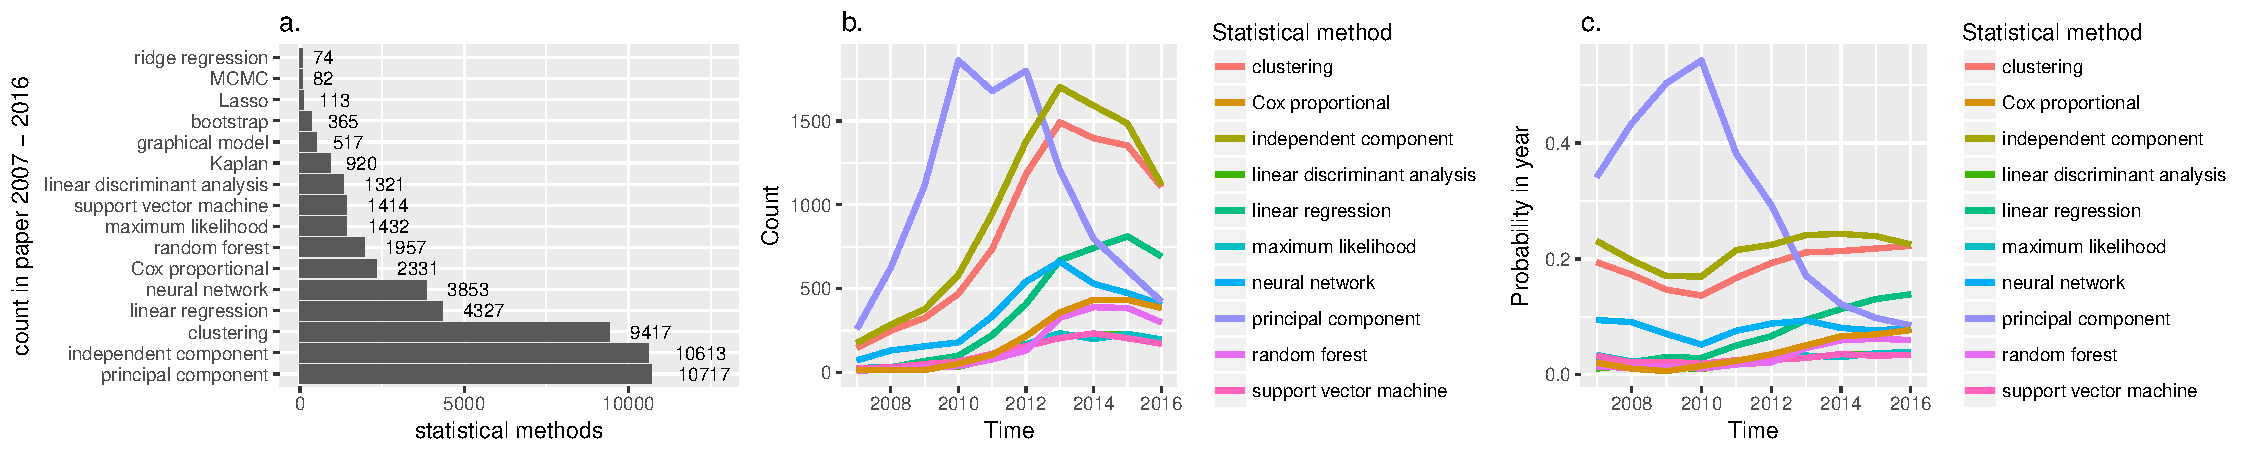
\includegraphics[scale=.4]{p1.pdf}
\centering
\caption{Total count and time trend of common statistical methods 2007-2016. (a) Total counts of each methods over the decade. (b) Year count plotted against year. (c) Year count proportion for each method within each year plotted against year.}
\label{fig:digraph}
\end{figure}

As for the time trend, we could fit linear splines over each word. The starting point of each method was below 400 (Figure 1b). We noticed that the principal component analysis increased in the initial four years with 250 more mentioning each year, then fluctuated and experienced a drop to nearly the starting level. Independent component analysis and clustering had a similar trend over the years: increased from 300 to the highest point around 1500 and 1700 at 2013, then started to decrease. All the other methods shared similar "increasing then decreasing" trend with turning points between the year 2013 and 2015, and the decreasing rate was 5\%.

The data were normalized by considering the total number of counts each year. We calculated the count proportion one method took within one year, used these data to plot the time trend (Figure 1c). The fluctuation of principal component analysis disappeared and it had the most noticeable change. Starting from a proportion of 35\%, this method accounted for more than 50\% of all statistical methods at 2010, then decreased dramatically to less than 10\% at 
2016. Independent component analysis and clustering stayed at the 20\% level with less than 5\% fluctuation. Linear regression enjoyed a steady increase from a value close to 0 at the start point to 15\% at 2016. Among all machine learning based algorithm, neural network had the most significant share at around 10\%. Random forest and support vector machine increased slightly to 5\% in the end. 

The first 30 words with the highest probability were selected and we were able to set the topics by observing those words: laboratory science, community survey, natural disaster, infectious disease and population network (Figure 2b). These coincided with the journals of PLoS Current. For each paper, we defined its topic as the one with maximum posterior probability.

By using regular expressions of all words from the dictionary, we found that 48 papers had these keywords in their method part. Among them, 11 papers were defined as community survey; 5 infectious disease; 11 laboratory science; 8 natural disaster; 13 population network. The new dictionary contained 8 statistical method: "linear regression", "bootstrap", "maximum likelihood", "MCMC", "neural network", "clustering", "principal component" and "Kaplan".

\begin{figure}[ht]
\begin{minipage}{\textwidth}
  \begin{minipage}[b]{0.51\textwidth}
      \centering
    \tiny
\begin{tabular}{|l|l|l|l|l|}
\hline
Topic 1                                                                                                              & Topic 2                                                                                                                       & Topic 3                                                                                                                         & Topic 4                                                                                                                  & Topic 5                                                                                                                           \\ \hline
\begin{tabular}[c]{@{}l@{}}animal\\ days\\ muscle\\ testing\\ statistical\\ control\\ genotype\\ tissue\end{tabular} & \begin{tabular}[c]{@{}l@{}}community\\ local\\ survey\\ government\\ district\\ response\\ services\\ collection\end{tabular} & \begin{tabular}[c]{@{}l@{}}mortality\\ earthquake\\ injuries\\ hurricane\\ disasters\\ deaths\\ severity\\ natural\end{tabular} & \begin{tabular}[c]{@{}l@{}}outbreak\\ transmit\\ virus\\ epidemic\\ incidence\\ incubated\\ rate\\ infected\end{tabular} & \begin{tabular}[c]{@{}l@{}}individual\\ interview\\ population\\ network\\ trees\\ household\\ social\\ participants\end{tabular} \\ \hline
\begin{tabular}[c]{@{}l@{}}laboratory\\ science\end{tabular}                                                         & \begin{tabular}[c]{@{}l@{}}community\\ survey\end{tabular}                                                                    & \begin{tabular}[c]{@{}l@{}}natural\\ disaster\end{tabular}                                                                      & \begin{tabular}[c]{@{}l@{}}infectious\\ disease\end{tabular}                                                             & \begin{tabular}[c]{@{}l@{}}population\\ network\end{tabular}                                                                      \\ \hline
\end{tabular}
    \captionof*{table}{a}
  \end{minipage}
  \hfill
  \begin{minipage}[b]{0.49\textwidth}
    \centering
    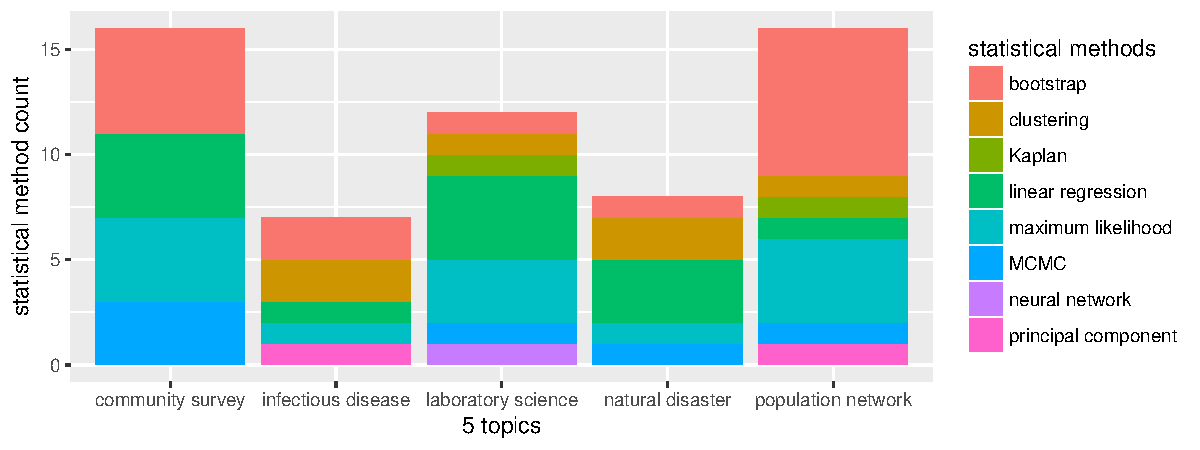
\includegraphics[scale=.4]{p2.pdf}
    \captionof*{figure}{b}
    \end{minipage}
  \end{minipage}
  \caption{Topic model: topic selection and statistical method distribution over topics. (a) Words among top 30 words sorted by descending order of posterior probability that were used to determine topics. (b) Common statistical methods distribution over 5 topics}
\end{figure}

The plot (Figure 2b) showed that bootstrap, maximum likelihood and linear regression were used in all different fields. For population network, the most often used method was bootstrap, then maximum likelihood, which in total took 67\% of all methods. It also had the largest number of different methods 7. For community survey, bootstrap, linear regression, maximum likelihood and MCMC shared the methods almost equally. For laboratory science, linear regression and maximum likelihood methods accounted for more than 60\%. There were not enough papers for the other two topics to make an accurate inference. 

In conclusion, principal component analysis, independent component analysis and clustering were the most common techniques. All methods experienced first increasing then decreasing trend in raw count. When observing the trend of proportion that one method took within one year, that is, the raw count of one method divided by the total count of all method of specific year, principal component analysis changed dramatically, while linear regression, support vector machine and random forest increased steadily over the ten-year period. The methods used for all fields were bootstrap and linear regression. It was more common to use bootstrap in population network research. For scientific research based on laboratory experiment, linear regression and maximum likelihood methods were used more often. 



\section{Discussion}

The exploratory data analysis brought us a clear overview of the time trend of different statistical methods. However, there are certain drawbacks. When creating keywords dictionary, we did not set quantifiable standards for "most common statistical methods". Some keywords might not exist as a statistical term, such as "neural network". More complicated statistical models can be applied to view the relationship of time and topics. However, the only feature is time, so regression analysis is hard to conduct, or the results would be similar to the splines. Plotting is the most straightforward way. Moreover, no function in “rplos” can search the words in method parts, but the appearance in the abstract can be representative. 

The topic model correctly specified the topics within "PLoS Current" directory, containing journals from different fields. For the output words from the topic model, we noticed there were special symbols that had only ASCII form and appeared to be blanks. These should be removed from the training data. We only removed part of the functions used in Latex. A more detailed Latex stopwords should be created. We tried stemming process before building the model, but the process truncated the words too much, which made it hard for us to associate the words back. This resulted in the repetition in final words output, such as plural forms and words with the same meaning but a different part of speech. The original idea was to use the topic model to get statistical method and word distribution directly using the text file. However, as not all papers are statistical papers, the topics are field-specific when looking at "method" part. The modeling procedure is intriguing and we did find out different fields. The future analysis would be adding time as a variable into the topic model \cite{topicovertime}, created a more extensive statistical-method-based dictionary and train the topic model under these constraints. 


\begin{thebibliography}{12}
\bibitem{plos} 
PLoS introduction,
\texttt{https://www.plos.org/who-we-are}

\bibitem{methodbook} 
Trevor Hastie, Robert Tibshirani, Jerome Friedman.
\textit{The Elements of Statistical Learning - Data Mining, Inference, and Prediction. 2nd edition.}. 
Springer, 2009.

\bibitem{words}
Common English words,\texttt{https://github.com/dwyl/english-words/blob/master/words.txt}

\bibitem{rplos} 
Scott Chamberlain, Carl Boettiger and Karthik Ram (2016). 
\textit{rplos: Interface to the Search 'API' for 'PLoS' Journals} \texttt{https://CRAN.R-project.org/package=rplos}

\bibitem{stringr}
Hadley Wickham (2017). 
\textit{stringr: Simple, Consistent Wrappers for Common String Operations. R package version 1.2.0.} \texttt{https://CRAN.R-project.org/package=stringr}

\bibitem{ggplot2}
H. Wickham. 
\textit{ggplot2: Elegant Graphics for Data Analysis.}
Springer-Verlag New York, 2009.

\bibitem{tm}
Ingo Feinerer, Kurt Hornik, and David Meyer (2008).
\textit{Text Mining Infrastructure in R.}
Journal of Statistical Software 25(5): 1-54.

\bibitem{tidytext}
Silge, Julia and Robinson, David
\textit{tidytext: Text Mining and Analysis Using Tidy Data Principles in R.}
The Journal of Open Source Software

\bibitem{dplyr}
H. Wickham, R. Francois, L. Henry and K. Müller (2017). 
\textit{dplyr: A Grammar of Data Manipulation. R package version 0.7.4.} \texttt{https://CRAN.R-project.org/package=dplyr}

\bibitem{topicmodels}
Grün B and Hornik K (2011). 
\textit{topicmodels: An R Package for Fitting Topic Models.}
Journal of Statistical Software. 

\bibitem{topicovertime}
Xuerui Wang, Andrew McCallum.
\textit{Topics over Time: A Non-Markov Continuous-Time Model of Topical Trends}
12th ACM SIGKDD international conference on Knowledge discovery and data mining, Pages 424-433. Philadelphia, PA, USA, 2006 

\bibitem{LDA}
David M. Blei, Andrew Y. Ng, Michael I. Jordan,
\textit{Latent Dirichlet Allocation}
Journal of Machine Learning Research 3 (2003) 993-1022
Submitted 2/02; Published 1/03

\end{thebibliography}

\end{document}